Wybór technologii ma duży wpływ na różne aspekty projektu programistycznego.
Od niego zależy na jakich platformach może zostać on tworzony i uruchamiany.
Dobre biblioteki potrafią znacząco ułatwić tworzenie oprogramowania pozwalając skupić się programistom na tworzeniu funkcjonalności aplikacji.
Nie ma potrzeby tworzyć nowego systemu wyświetlania interfejsu użytkownika na potrzebę każdego projektu osobno, gdy jest wybór wielu bardzo dobrze wspieranych technologii na każdą platformę.

Przy wyborze technologii dla aplikacji oprócz funkcjonalności zostały wzięte pod uwagę:
\begin{itemize}
    \item \textbf{Dobrze napisaną dokumentację:} Obsługa biblioteki programistycznej jest dużo łatwiejsza, gdy jej twórca udostępnia dobrze napisane materiały jak z niej korzystać.
    \item \textbf{Otwarty kod źródłowy:} Projekty open source udostępniają swój kod - nawet w momencie, kiedy dokumentacja nie jest idealna możemy zobaczyć jak dana funkcja działa.
    \item \textbf{Aktywne utrzymywanie:} Biblioteka bez aktualizacji do nowszych wersji może sprawiać problemy w postaci luk bezpieczeństwa lub problemami z kompatybilnością.
    \item \textbf{Dojrzała technologia:} Korzystając z kodu tworzonego i używanego od wielu lat można spodziewać się większej ilości przykładowych użyć, dopracowanego interfejsu projektu oraz pozbawionego błędów działania.
\end{itemize}

\subsection{Język programowania}

Jest to kluczowy wybór, ma wpływ na większość następnie wybranych technologii.
Język programowania ma wpływ na wydajność aplikacji, trudność jej tworzenia oraz późniejszego utrzymania.
Dzięki wyborze popularnego języka można mieć dostęp do bardzo szerokiej gamy gotowych bibliotek rozwiązujących popularne problemy jak komunikacja z serwerami czy zapisywanie i odczytywanie formatu JSON.

\subsubsection{C\#}

Wieloparadygmatowy język ogólnego przeznaczenia tworzony przez Microsoft od ponad 20 lat \cite{csharp}.
Jest on kompilowany przed uruchomieniem co daje przewagę wydajności nad językami interpretowanymi.
Można obecnie pisać w nim aplikacje na komputery stacjonarne, telefony, przeglądarki czy serwery.
Posiada narzędzie do zarządzania bibliotekami NuGet \cite{nuget} pozwalająca na łatwe dodanie zależności do projektu.

\subsection{Platforma programowa}

Wiele języków programowania posiada swoją platformę programistyczną - jest to narzędzie za pomocą którego można tworzyć projekty, zarządzać bibliotekami, budować i uruchamiać aplikację.

\subsubsection{.NET Core}

.NET Core to platforma programistyczna opracowana przez firmę Microsoft, stanowiąca otwartoźródłowe i wieloplatformowe środowisko do tworzenia różnorodnych typów aplikacji, w tym aplikacji internetowych, usług sieciowych oraz aplikacji konsolowych.
Obsługuje wiele języków z których najpopularniejszy jest C\# \cite{dotnet}.
Jej struktura podzielona jest na moduły takie jak środowisko uruchomieniowe, kompilacja czy wbudowane biblioteki.

\subsection{Interfejs użytkownika}

W celu zapewnienia użytkownikom szybkiego wykonywania operacji wybrano jako docelową platformę komputer stacjonarny.
Zawęża to wybór możliwych technologii tworzenia interfejsu.
Rozważone zostały dwie technologie - Avalonia UI \cite{AvaloniaUI} oraz WPF \cite{wpf}.
Pierwsza z nich jest nowsza i aktywnie rozwijana, może działać na wielu platformach w przeciwieństwie do rozwiązania stworzonego przez Microsoft. 
W momencie decydowania o interfejsie użytkownika jednak pojawiały się błędy w funkcjonalnościach potrzebnych do działania projektu.

\subsubsection{Windows Presentation Foundation}

Jest to platforma graficzna opracowana przez firmę Microsoft, została po raz pierwszy wprowadzona jako część .NET Framework w 2006 roku \cite{wpfHistory}. 
Umożliwia tworzenie bogatych interfejsów użytkownika dla aplikacji stworzonych na system Windows.
Elementy są wyświetlane wektorowo co pozwala na dowolne skalowanie elementów. 
Widoki są definiowane w formacie XAML co pozwala na oddzielenie logiki biznesowej od warstwy prezentacji.
Platforma ta umożliwia powiązanie elementów interfejsu z danymi aplikacji co pozwala na szybkie aktualizowanie widoku z najnowszymi wynikami.

\subsubsection{Nodify}
\begin{figure}[H]
    \centering
    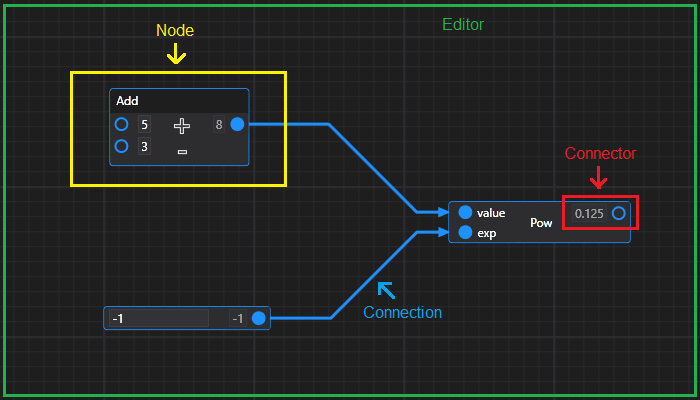
\includegraphics[width=0.8\linewidth]{./images/Picture7.png}
    \caption{Opis elementów edytora węzłów \cite{node}.}
    \label{fig:nodify}
\end{figure}

Biblioteka Nodify \cite{nodify} jest otwartoźródłowym projektem implementującym edytor węzłowy \autoref{fig:nodify} dla biblioteki WPF. 
Poprawna implementacja tego projektu daje możliwość dodawania bloczków i łączenie ich w ciągi. 
Wystarczy zaimplementować co dzieje się z danymi w węzłach oraz jak zostają one przekazywane dalej żeby mieć funkcjonalny interfejs użytkownika. 

\subsubsection{WPF UI}
\begin{figure}[H]
    \centering
    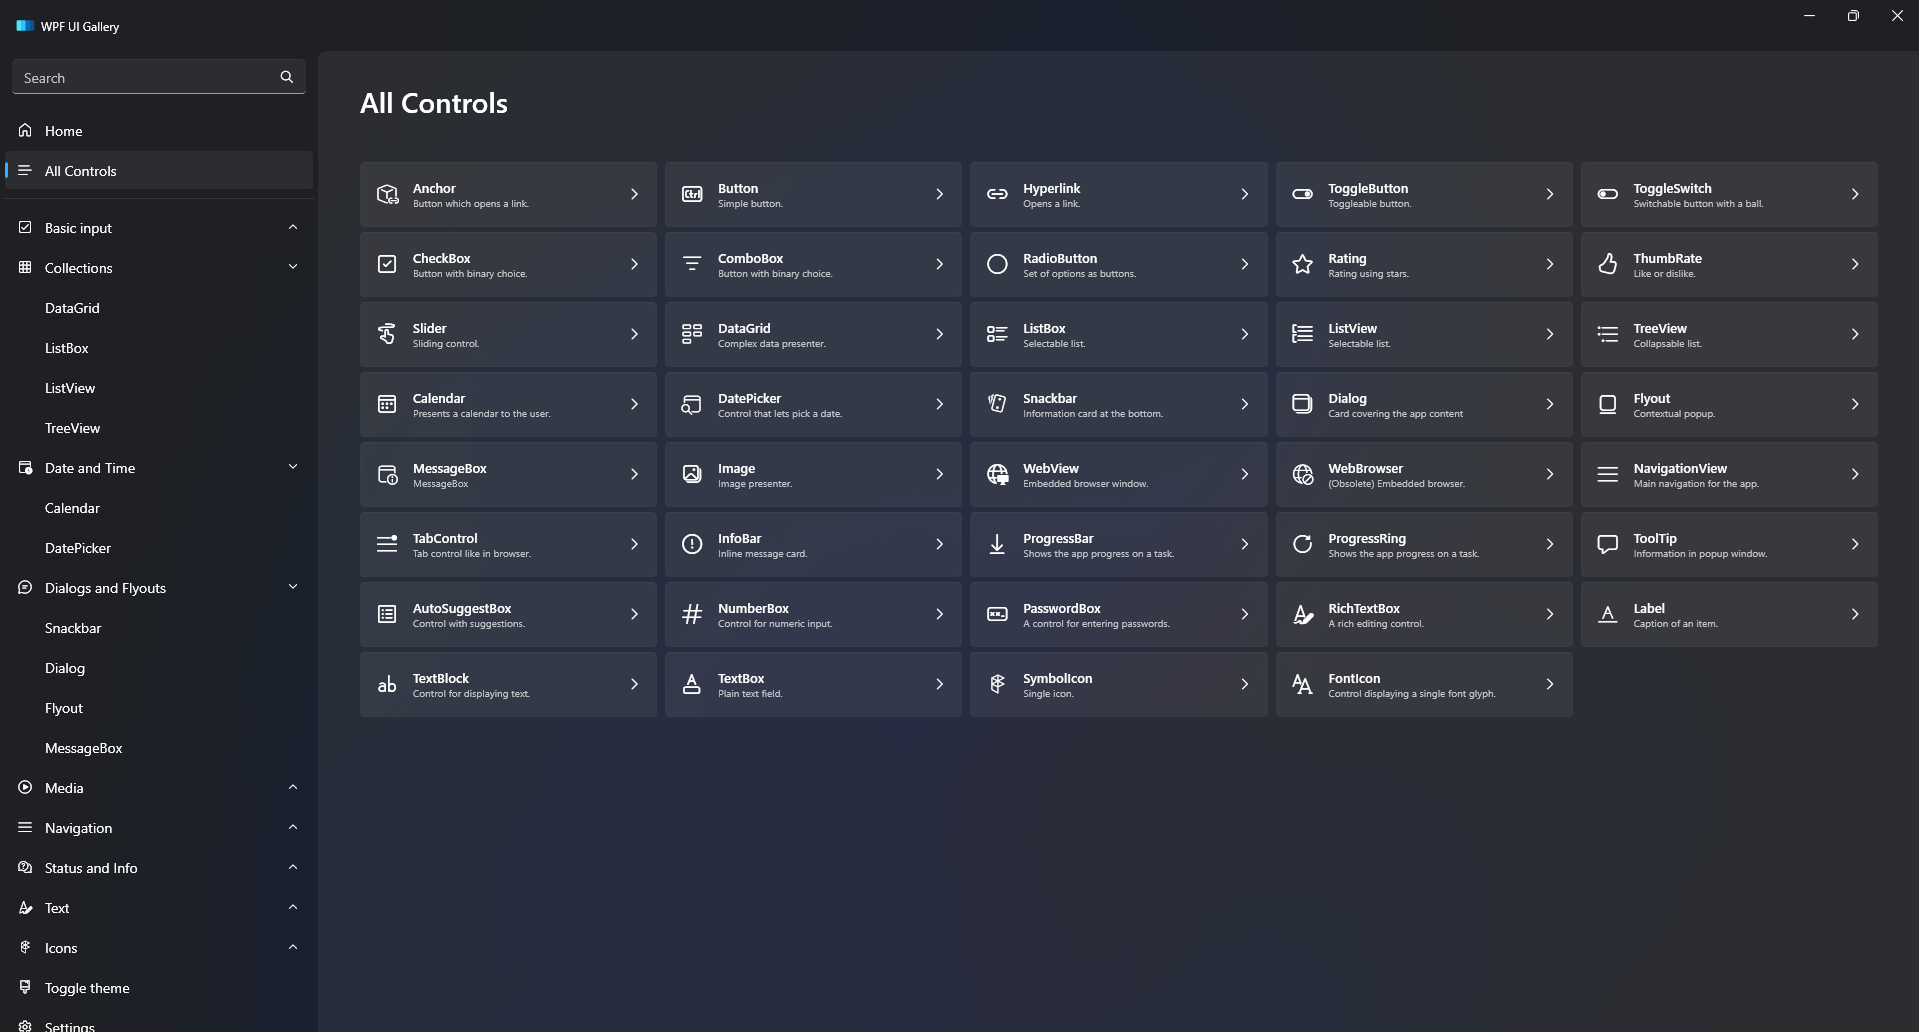
\includegraphics[width=0.9\linewidth]{./images/Picture8.png}
    \caption{Galeria elementów WPF UI. Opracowanie własne.}
    \label{fig:wpfui}
\end{figure}

Biblioteka WPF UI \cite{wpfui} modyfikuje i dodaje elementy interfejsu używane w Windows Presentation Foundation \autoref{fig:wpfui}. 
Jest ona zgodna z systemem projektowania interfejsu Fluent 2 \autoref{fig:winui3} od Microsoftu używanego w wielu aplikacjach dla systemu Windows 11. 
Pozwala to na utrzymanie nowoczesnej stylistyki w projekcie bez potrzeby tworzenia skomplikowanych stylów imitujących WinUI 3 od zera.

\begin{figure}[H]
    \centering
    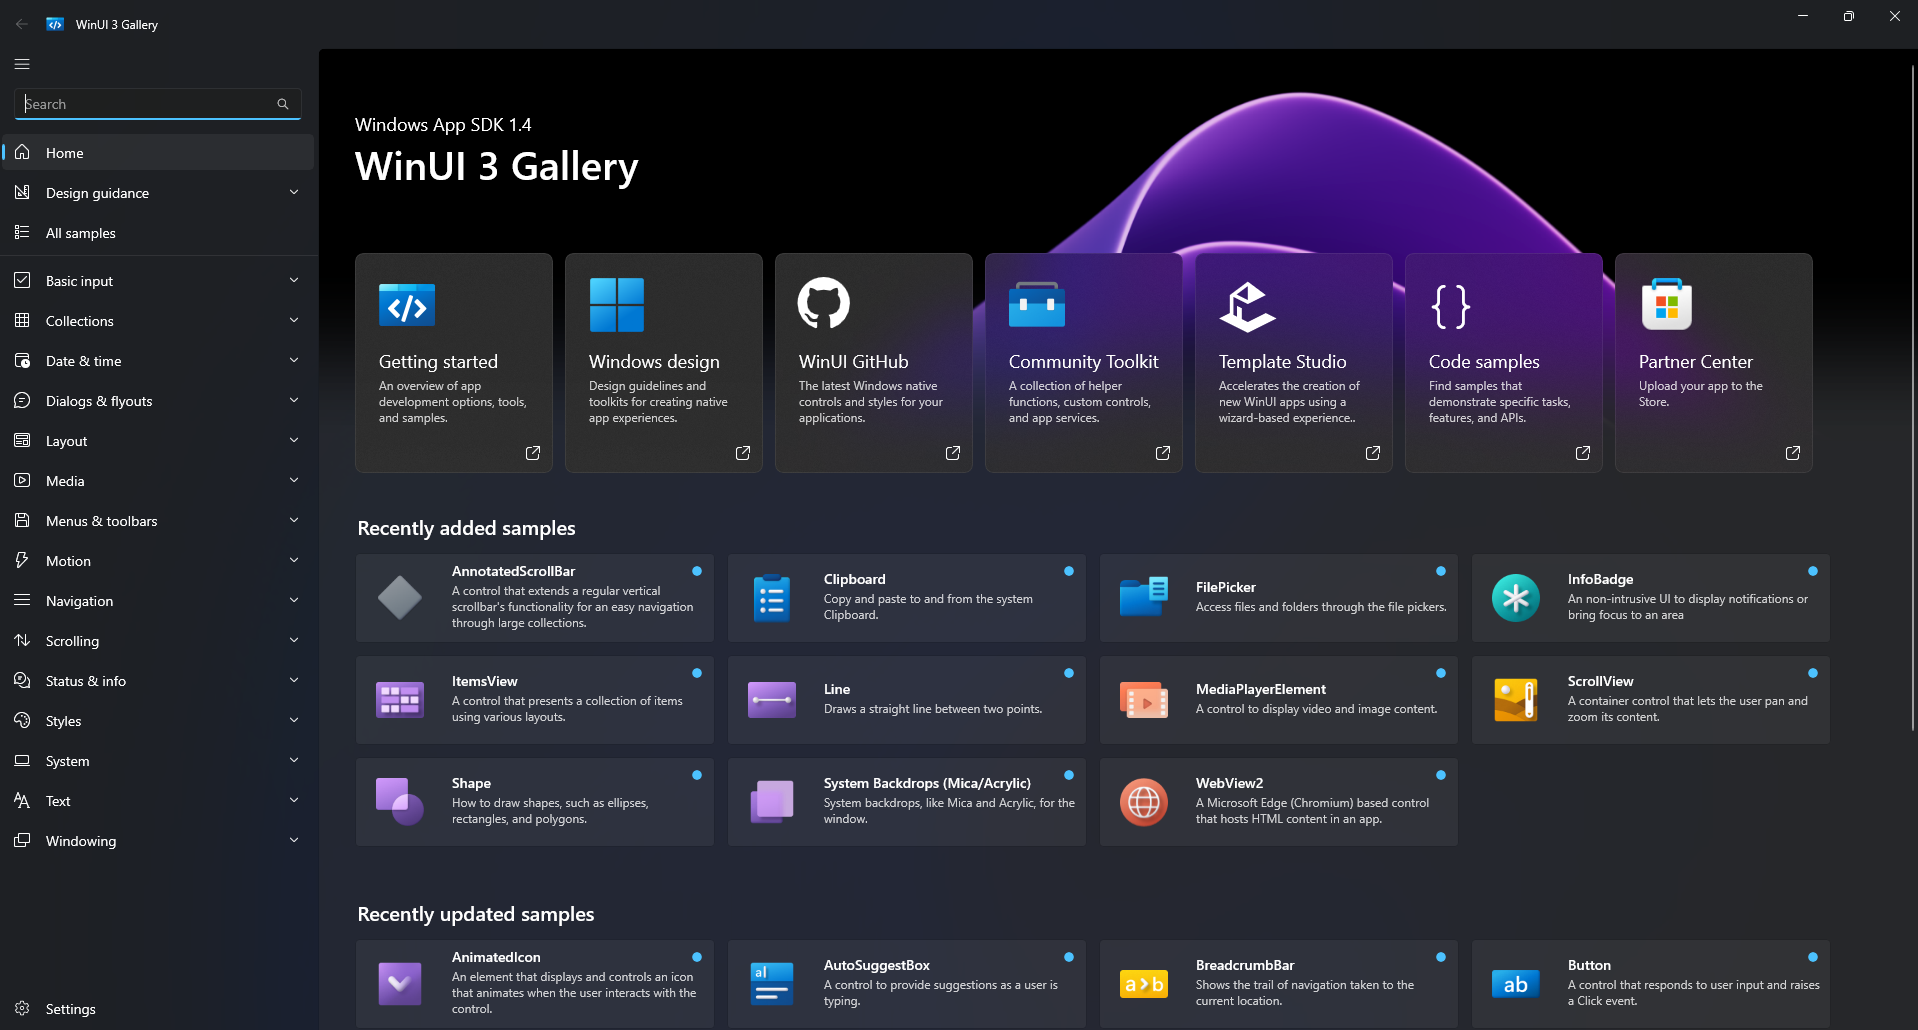
\includegraphics[width=0.9\linewidth]{./images/Picture9.png}
    \caption{Galeria elementów WinUI 3. Opracowanie własne.}
    \label{fig:winui3}
\end{figure}

\subsection{Biblioteka do przetwarzania obrazów}
Jedną z popularnych bibliotek do przetwarzania obrazów jest OpenCV.
Nazwa to skrót od \textit{Open Source Computer Vision Library} i wskazuje, że jest to darmowy i otwartoźródłowy projekt skupiony na przetwarzaniu obrazów oraz widzeniu maszynowym.
Pakiet ten dostępny jest dla systemów Windows, macOS i Linux. 
Został stworzony w Intel Research Labs w 1999 roku \cite{opencvHistory}. Biblioteka ta jest napisana w języku C\++ i kładzie duży nacisk na prędkość obliczeń. Pozwala ona na przetwarzanie obrazów, wideo, posiada zaawansowane algorytmy wykrywania obiektów, klasyfikacji oraz wiele operacji korzystajacych z sieci neuronowych.

\subsubsection{OpenCvSharp}

Projekt jest tworzony w języku C\# więc nie możemy bezpośrednio odwoływać się do biblioteki OpenCV. Powstało kilka projektów które opakowują oryginalny pakiet w metody którymi możemy się odwołać bez problemu z kodu w platformie .NET. Dwie najpopularniejsze biblioteki tego typu to EmguCV \cite{emgucv} oraz OpenCvSharp \cite{opencvsharp}. 
Obie cieszą się dużym wsparciem społeczności lecz pierwsza z nich jest mniej zgodna z API oryginalnej paczki oraz jest wolniejsza.

\subsection{Biblioteka do walidacji}

W interfejsie użytkownika należy wprowadzić dane, nie możemy założyć że będą one poprawne.
Wszystkie wejścia trzeba zabezpieczyć tak by użytkownik nie mógł przerwać działania programu i zawsze wiedział dlaczego jego operacje się nie wykonują.

\subsubsection{Fluent Validation}

Biblioteka Fluent Validation \cite{fluentvalidation} pozwala na proste ustalanie reguł według których ocenia czy dane są prawidłowe oraz przypisanie odpowiedniej wiadomości błędu gdy nie są. Paczka ta jest przejrzysta oraz posiada dobrą dokumentację i wiele przykładów implementacji. 

\subsection{Biblioteka do serializacji}

Serializacja jest potrzebna gdy chcemy zapisać stan naszej aplikacji lub wysłać jakieś dane. Dla wygody użytkownika należy wprowadzić system zapisywania i wczytywaniu plików, żeby mógł wrócić do wcześniej stworzonych ciągów operacji oszczędzając jego czas. 

\subsubsection{Json.NET}

Newtonsoft.Json \cite{Newtonsoft.Json} to najpopularniejsza biblioteka do obsługi plików Json w galerii paczek NuGet \cite{jsonMostPop}. 
Pozwala na serializowanie obiektów i deserializowanie Json'a do obiektów zachowując złożone struktury obiektów i kolekcje oraz posiada wiele parametrów za pomocą których można dopasować jego wyniki do większości zastosowań. 

\subsection{Środowisko deweloperskie}

Odpowiednie środowisko może znacząco przyśpieszyć pracę nad projektem programistycznym. 
Nowoczesne IDE (ang. \textit{Integrated Development Environment}) zamykają nawiasy, pomagają w poprawianiu błędów, refaktoryzacji i proponują automatyczne uzupełnienia zmiennych czy metod biorąc pod uwagę kontekst kodu w plikach.
Ważne jest też zadbanie o kontrolę wersji w celu zapisywania stanu projektu oraz śledzeniu zmian zachodzących w nim.

\subsubsection{Microsoft Visual Studio}
\begin{figure}[H]
    \centering
    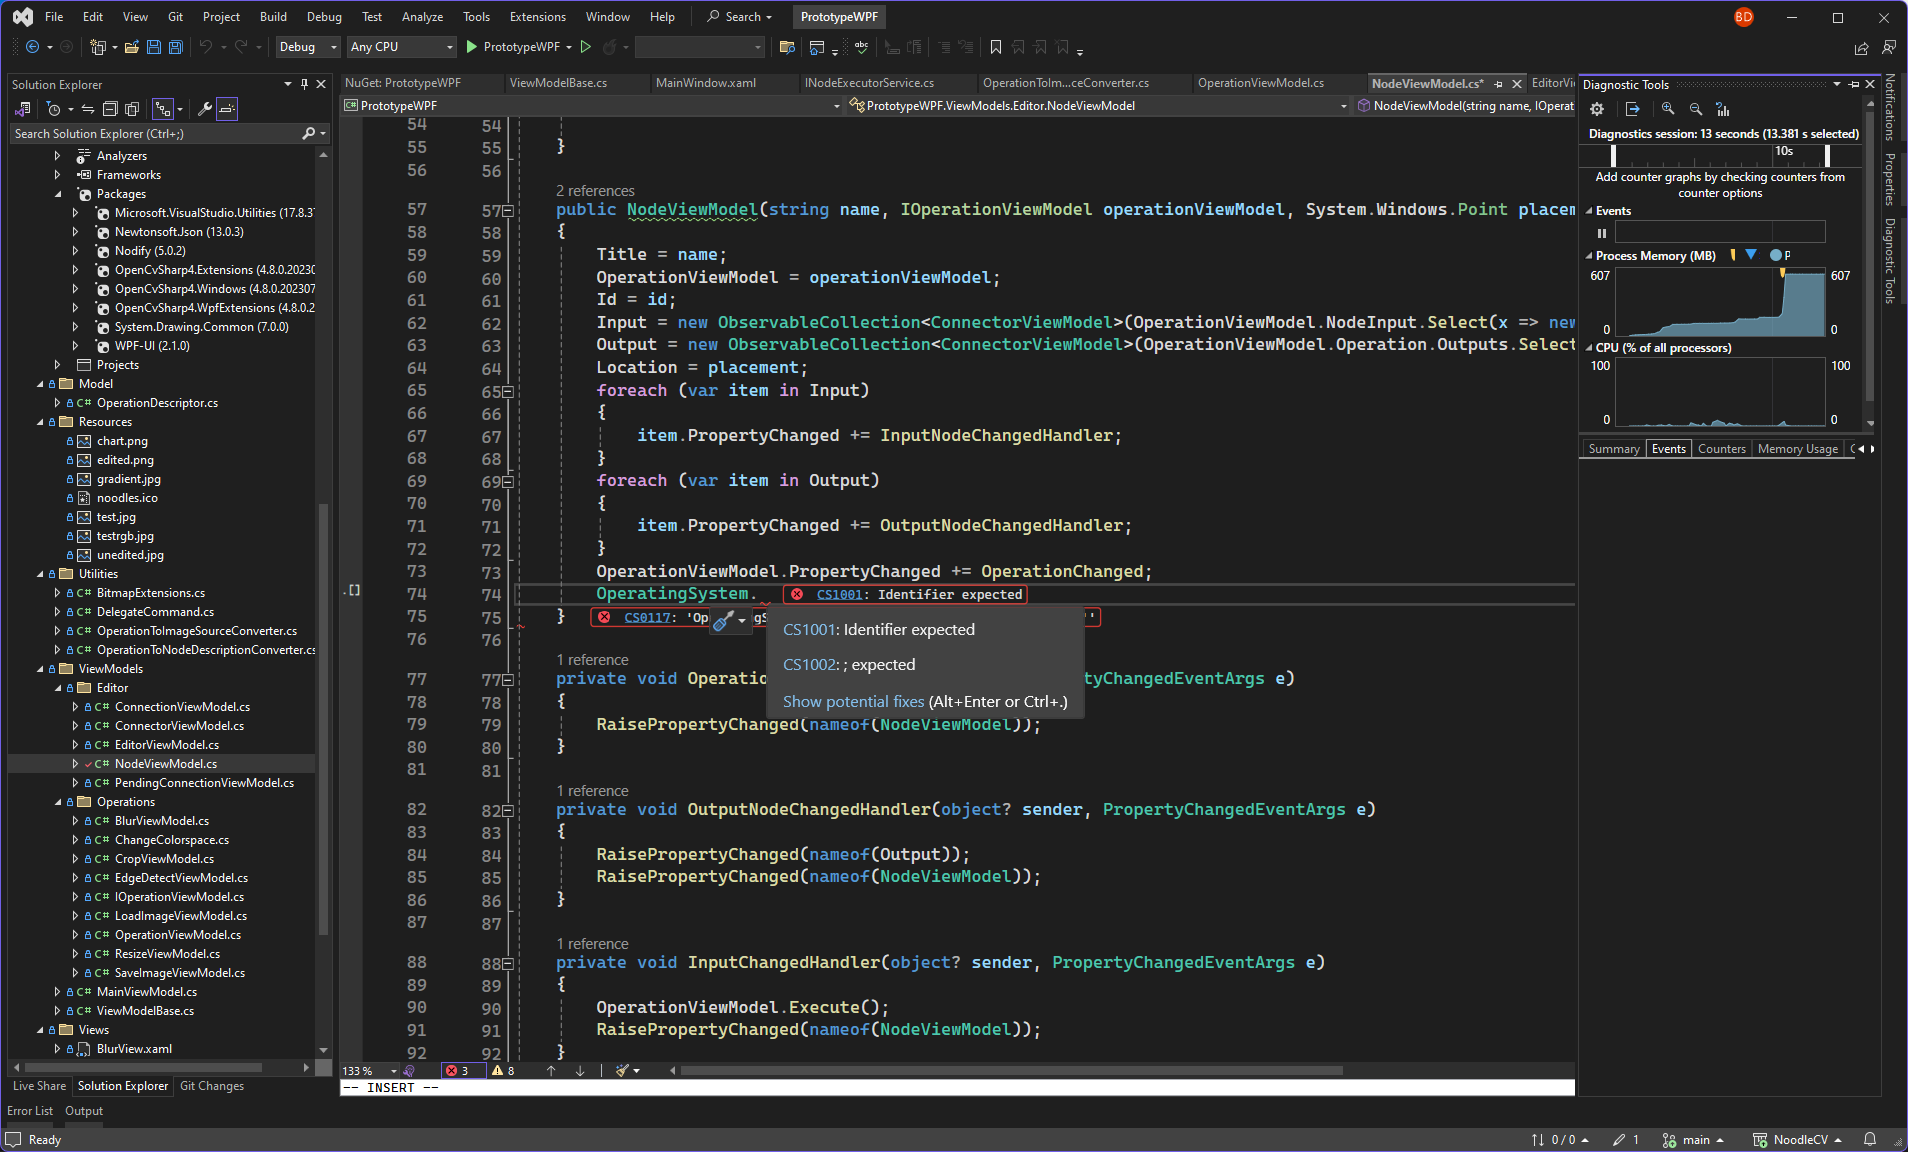
\includegraphics[width=1\linewidth]{./images/Picture10.png}
    \caption{Interfejs programu Visual Studio. Opracowanie własne.}
    \label{fig:visual}
\end{figure}

Microsoft Visual Studio \cite{visualstudio} to zintegrowane środowisko programistyczne (IDE) opracowane i wydane przez firmę Microsoft. Jest przeznaczone do tworzenia aplikacji komputerowych, w tym aplikacji internetowych, aplikacji mobilnych, aplikacji desktopowych i aplikacji konsolowych. Posiada wiele gotowych zestawów narzędzi do pobrania dla specyficznych typów programów, a jego funkcjonalność dodatkowo można rozszerzać dodatkami pobieranymi z internetu.

\subsubsection{Git}

Git \cite{git} to system kontroli wersji oparty na rozproszeniu danych (ang. \textit{distributed version control system - DVCS}), opracowany przez Linusa Torvaldsa. 
Jest przeznaczony do śledzenia zmian w plikach i folderach, a także do współpracy nad projektami w czasie rzeczywistym. 